% Description of slam, common approaches and frameworks

\chapter{Simultaneous Localization and Mapping (SLAM)}
\label{ch:slam}

Simultaneous Localization and Mapping (\textbf{SLAM}) or Concurrent Mapping and Localization (\textbf{CML}) is one of the most fundamental problems in robotics \citeslam{Durrant-Whyte2006, Thrun2005, Tobergte2013}. It tackles the task of placing a robot in an unknown environment and being able to build a map while keeping track of the robot's own position on that map.

Since SLAM is one of the core features of mobile robotics, its applications range in the same field such as ground, indoor, underwater or air vehicles (\autoref {fig:slam}).
\begin{figure}[htb]
  \centering
  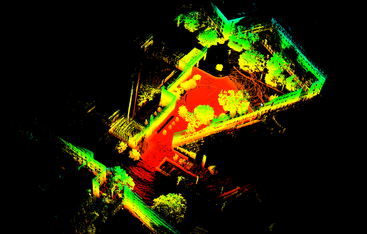
\includegraphics[width=\linewidth]{pictures/03/3dslam}
  \caption{3D example of SLAM techniques on the PEV}
  \label{fig:slam}
\end{figure}  


For its nature, SLAM is considered to be one of the toughest challenges of mobile robotics \citeslam{Burgard2017e, Thrun2005} and it is often referred as a \textbf{chicken--and--egg} problem:
\begin{itemize}
  \item In order for a robot to correct errors from odometry and localize in the environment it needs a map.

  \item In order to build a map, the robot needs to know its position and orientation with respect to the environment.
\end{itemize}

This interdependence between both problems is why they have to be approached at the same time, thus being named 'Simultaneous'.

SLAM is seen as the 'holy grail' of AVs and mobile robots in general \citeslam{Durrant-Whyte2006}, since once a robust method of building rich maps is found, it will allow for fully autonomous vehicles.

In fact, the SLAM problem has been solved in the theoretical plane, where many equally valid variants can be found; the problem arises when those algorithms are applied in real--life systems.

\section{SLAM fundamentals}

\subsection{Probabilistic Robotics}

The approach to SLAM is generally done in terms of probability instead of using single "best guess" values. This manner of tackling SLAM (and many other fields in mobile robotics) results to be very useful since neither sensors nor actuators are noise--free. By integrating those uncertainties into the models, controls can be made more robust, thus improving the performance of the robot.

The core of probabilistic robotics is \textbf{state estimation}, that is estimating environment and internal variables using sensor data. 

Denoting time with letter $t$, the state and environmental variables can be defined as \citeslam{Thrun2005, Tobergte2013}:
\begin{itemize}
  \item \textbf{State}: State is usually denoted with letter $x$ and is composed of position and orientation (relative to global frame), more commonly called \textbf{pose}. In flat navigation, the state comprises the tuple $(x\,\,y\,\,\theta)$. Thus, the state at time $t$ is denoted as $x_t$, and the collection of states from time $0$ to $t$, namely the \textbf{path}, is:
  \begin{equation}
    X_t = \{x_0, x_1, x_2,\ldots,x_t \}
    \label{eq:state}
  \end{equation} 

  Moreover, states can be \emph{complete} or \emph{incomplete}. A state is called \emph{complete} when the prior knowledge of state, control and perception does not add more information. However, in real--life situations, not all aspects of the robot are known, being that called \emph{incomplete}.

  % Mention chapter 2
  \item \textbf{Control actions}: Control actions change the state of the system (\eg, manipulation, forward movement) and data associated to these actions contain information on how the state changes. One of the most common sources of data is \emph{odometry} (\autoref{sub:perception}). Even though the sources of odometry are sensors, they measure the change of state, being equally valid for the purpose.
  
  Control data is usually denoted with $u$, and $u_t$ denotes the action that brings the system from state $x_{t-1}$ to $x_t$. Actions are collected in the vector:
  \begin{equation}
    U_t = \{u_0, u_1, u_2,\ldots,u_t \}
    \label{eq:actions}
  \end{equation}   

  \item \textbf{Environment measurements}: Sensors such as lidars or camera perform \emph{observations} to gain knowledge of the state of the system. Measurement data is denoted with $z$ and $z_t$ corresponds to a specific measurement at time $t$. $Z_t$ will denote the collection of all measurements from $0$ 0 to $t$:
  \begin{equation}
    Z_t = \{z_0, z_1, z_2,\ldots,z_t \}
    \label{eq:env}
  \end{equation}  
\end{itemize}  

Once the main variables have been defined, they are usually gathered into a probability distribution called \emph{belief} or \emph{state of knowledge}, that represents the pose at time $t$ taking into account the previous data:
\begin{equation}
  bel(x_t) = p(x_t|z_{1:t},u_{1:t})
  \label{eq:belief}
\end{equation}  

There is a variant of the belief, called prediction, that estimates the pose without taking into account the latest sensor measurement and that is denoted $\overline{bel}(x_t)$:
\begin{equation}
  \overline{bel}(x_t) = p(x_t|z_{1:t-1},u_{1:t})
  \label{eq:prediction}
\end{equation}  

Having defined these variables, now the Bayes filter can be deduced.

\subsection{Bayes filter}

The bayes filter is a technique to peform state estimation, based on previous beliefs and sensor measurements. It is of essential importance in Probabilistic Robotics, since it is the basis for practically all other approaches in the field \citeslam{Burgard2017e, Durrant-Whyte2006}.

The goal is to determine the law that provides the probability distribution of the belief at time $t$, $bel(x_t)=p(x_t|z_{1:t},u_{1:t})$. For that we start with the combined probability $p(x_t,z_{1:t},u_{1:t})$ and apply the \textbf{Bayes rule} (hence the name):

\begin{equation}
  \begin{split}
    p(x_t,z_{1:t},u_{1:t}) & = p(z_{1:t-1},u_{1:t})\cdot p(z_t|z_{1:t-1},u_{1:t})\cdot p(x_t|z_{1:t},u_{1:t})\\
                           & = p(z_{1:t-1},u_{1:t})\cdot p(x_t|z_{1:t-1},u_{1:t})\cdot p(z_t|x_t,z_{1:t-1},u_t)
  \end{split}  
  \label{eq:bayesded}
\end{equation}  

Considering that $p(z_{1:t-1},u_{1:t})$ appears on both sides, it can be cancelled out. Then, reordering the elements of the equation:
\begin{equation}
  \begin{split}
    bel(x_t) = p(x_t|z_{1:t},u_{1:t}) & = \frac{p(z_t|x_t,z_{1:t-1},u_t)\cdot p(x_t|z_{1:t-1},u_{1:t})}{p(z_t|z_{1:t-1},u_{1:t})} \\ 
                                      & = \eta\cdot p(z_t|x_t,z_{1:t-1},u_t)\cdot \overline{bel}(x_t)
  \end{split}
  \label{eq:bayes}
\end{equation} 

Where parameter $\eta$ is called \emph{normalizer}. If it is assumed that the state is complete, then the measurement $z_t$ does not depend on the previous measurements or controls (this is called \textbf{Markov assumption}), thus it can be written:
\begin{equation}
  p(z_t|x_t,z_{1:t-1},u_t) = p(z_t|x_t)
  \label{eq:markovf}
\end{equation}  

As for the prediction, $\overline{bel}(x_t)$, applying the \emph{Theorem of Total Probability} the following is obtained:
\begin{equation}
  \begin{split}
    \overline{bel}(x_t) & = p(x_t|z_{1:t-1},u_{1:t})\\
                        & = \int p(x_t|x_{t-1},z_{1:t-1},u_{1:t})\cdot p(x_{t-1}|z_{1:t-1},u_{1:t})\cdot\mathrm{d}x_{t-1}
  \end{split}
  \label{eq:predicteq}  
\end{equation}  

Applying again the Markov assumption to $ p(x_t|x_{t-1},z_{1:t-1},u_{1:t})$, the resulting probability distribution is ($u_t$ is not cancelled since it carries information on the change from $x_{t-1}$ to $x_t$):
\begin{equation}
  p(x_t|x_{t-1},z_{1:t-1},u_{1:t}) = p(x_t|x_{t-1},u_t)
  \label{eq:markovs}
\end{equation}

As for the second term, $u_t$ can be taken away, as it does not predict state $x_{t-1}$:
\begin{equation}
  p(x_{t-1}|z_{1:t-1},u_{1:t}) = p(x_{t-1}|z_{1:t-1},u_{1:t-1}) = bel(x_{t-1})
  \label{eq:beliefprev}
\end{equation}

After these changes, \autoref{eq:bayes} is converted to:
\begin{equation}
  \begin{split}
    bel(x_t) & = \eta\cdot p(z_t|x_t)\cdot \overline{bel}(x_t)\\
                        & = \eta\cdot p(z_t|x_t)\cdot \int p(x_t|x_{t-1},u_t)\cdot bel(x_{t-1})\cdot\mathrm{d}x_{t-1}
  \end{split}
  \label{eq:bayesfinal}  
\end{equation} 

There are 2 important components in \autoref{eq:bayesfinal}, namely the \emph{measurement probability} $p(z_t|x_t)$, and the \emph{state transition probability} $p(x_t|x_{t-1},u_t)$. In \citeslam{Thrun2005}, \emph{observation models} and \emph{motion models} are provided, that allow to describe those probability distributions more accurately (\autoref{fig:bayesfilter}).
\begin{figure}[htb]
  \centering
  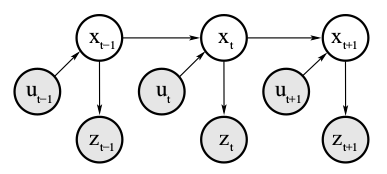
\includegraphics[width=\linewidth]{pictures/03/bayesfilter}
  \caption{Schematic of state determination using Bayes filter}
  \label{fig:bayesfilter}
\end{figure}

\subsection{Probabilistic robotics in SLAM}

When tackling SLAM, there is another variable that needs to be defined and it corresponds to the map features $m_i$, being $m$ the set of the $n$ features that compose the \textbf{map}:
\begin{equation}
  m = \{m_1,m_2,\ldots,m_n\}
  \label{eq:mapvar}
\end{equation}  

It is possible to add the map to the Bayes filter (\autoref{eq:bayesfinal}), since it can be considered as an extension of the state of the system. Therefore the bayes filter becomes:
\begin{equation}
  p(x_t,m|z_{1:t},u_{1:t}) = \eta\cdot p(z_t|x_t,m)\cdot p(x_t,m|z_{1:t-1},u_{1:t})
  \label{eq:bayesslam}  
\end{equation} 

In the probabilistic realm, there are 2 main forms of SLAM (\autoref{fig:approachslam}):
\begin{itemize}
  \item \textbf{Online SLAM}: This approach only seeks to recover the most recent pose and map as it is stated in \autoref{eq:bayesslam}. The previous poses and measurements get discarded in this approach.
  
  \item \textbf{Full SLAM}: In this case, instead of the current position, the whole path is estimated, yielding the following equation:
  \begin{equation}
    p(x_{0:t},m|z_{1:t},u_{1:t})
    \label{eq:fullslam}
  \end{equation}

  It is possible to derive the online SLAM from the full SLAM, by integrating all the poses throughout time \citeslam{Burgard2017e}:
  \begin{equation}
    p(x_t,m|z_{1:t},u_{1:t}) = \int\int\!\cdots\!\int p(x_{1:t},m|z_{1:t},u_{1:t})\mathrm{d}x_1\mathrm{d}x_2\ldots\mathrm{d}x_{t-1}
    \label{eq:onlinetofull}
  \end{equation}
\end{itemize}

\begin{figure}[htb]
  \centering
  \subfloat[Online SLAM]{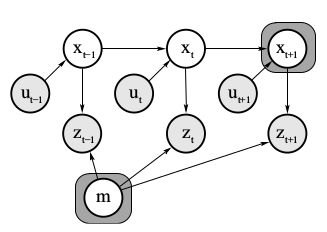
\includegraphics[width=.45\linewidth]{pictures/03/onlineslam}} \quad
  \subfloat[Full SLAM]{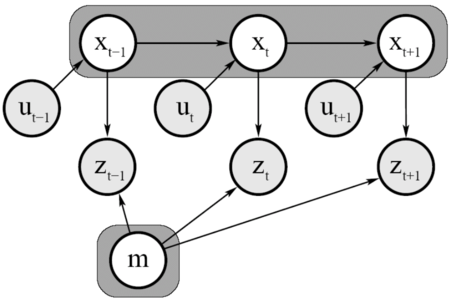
\includegraphics[width=.45\linewidth]{pictures/03/fullslam}}
  \caption{Schematic of the 2 SLAM approaches}
  \label{fig:approachslam}
\end{figure}

\subsection{SLAM dimensions}

The most usual differences among the SLAM algorithms are defined in the following paragraphs \citeslam{Tobergte2013}:

\begin{itemize}
  \item \textbf{Volumetric/Feature--based}: In volumetric SLAM, the map is sampled at realistic resolutions, thus the computational complexity grows notably. In feature--based maps, there are algorithms that process sensor readings and extract the key landmarks of the environment. The latter group is more data efficient, but it may lose some important sensor information.

  \item \textbf{Topological/Metric}: Topological maps are those that only characterize the environment with basic relationships, whereas metric ones provide more accurate descriptions of the surroundings (\autoref{fig:topometric}).
  \begin{figure}[htb]
    \centering
    \subfloat[Topological]{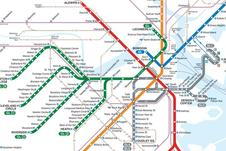
\includegraphics[width=.45\linewidth]{pictures/03/bsubway}} \quad
    \subfloat[Metric]{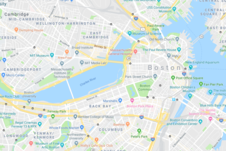
\includegraphics[width=.45\linewidth]{pictures/03/breal}}
    \caption[2 maps of Boston]{2 maps of Boston: Subway (Topological) vs Satellite (Metric)}
    \label{fig:topometric}
  \end{figure}
  

  \item \textbf{Known/Unknown correspondence}: Correspondence refers to matching sensed features from different timestamps. Some SLAM algorithms assume the identity of landmarks is known while others do not. The problem of determining those correspondences is known as \emph{data association} and it is one of the toughest challenges in SLAM.

  \item \textbf{Static/Dynamic}: The same way as it was described in localization (\autoref{sub:localization}), environments can be static if the environment remains the same over time, or dynamic if there are moving parts. Most of SLAM algorithms suppose static worlds.

  \item \textbf{Small/Large uncertainty}: Algorithms that allow for small uncertainties require that robots move along simple paths back and forth. If the path is more complex and there are multiple paths to return to the starting point, it will cause more uncertainty. In these cases the ability of the algorithm to perform \textbf{loop closure} correctly is crutial. Loop closure is the task of matching a previously visirted area with the current sensor readings \citeslam{Newman2005}. Today, most SLAM algorithms implement more or less sophisticated loop--closing modules. 

  \item \textbf{Active/Passive}: As in localization, when the SLAM algorithm is passive, it just observes to the movement of the robots and estimates the location and the map. In active SLAM, the algorithm itself takes control of the vehicle, resulting in more accurate maps. Nevertheless, the majority of SLAM approaches belong to the passive field.

  \item \textbf{Single/Multi--robot}: Most approaches use the single--robot assumption, though the multi--robot exploration is gaining adepts in the last years. In the latter form, robots are given relative positions to each other and a form of communication among them.
\end{itemize}

\section{SLAM varieties} \label{sec:varieties}

Having set the basics of the SLAM problem, it is time to describe the 3 main SLAM paradigms from which most of the algorithms stem: \textbf{Kalman filter SLAM}, \textbf{Particle filter SLAM} and \textbf{GraphSLAM}.

\subsection{Kalman Filter SLAM} \label{sub:ekf}

Kalman filter SLAM (more specifically Extended Kalman Filter (EKF)) is one of the earliest versions of SLAM \citeslam{Thrun2005,Tobergte2013}. As its name suggests it is based on Kalman filter approaches, which are methods devised by R.E. Kalman in the 1960s to solve the discrete linear filtering problem \citeslam{Bishop2001}. 

Kalman filter and its siblings assume that states can be modelled by gaussian distributions \citeslam{Stachniss2014a}:
\begin{equation}
  p(x) = det(2\pi\Sigma)^{-\frac{1}{2}}\cdot exp({-\frac{1}{2}(x-\mu)^T\Sigma^{-1}(x-\mu)})
  \label{eq:gauss}
\end{equation}  

Where $x$ is the state vector, $\mu$ is the mean vector and $\Sigma$ is the covariance matrix.

Kalman filter then models the state prediction and the measurement as:
\begin{gather}
  x_t = A_tx_{t-1} + B_tu_t + \epsilon_t \\
  z_t = C_tx_t + \delta_t 
  \label{eq:kfpred}
\end{gather}  
where $A_t$ is a $(n\times n)$ matrix that describes the evolution from $t-1$ to $t$ without controls, $B_t$ is a $(n\times l)$ matrix that describes the changes induced by control $u_t$, $C_t$ a $(k\times n)$ matrix that maps the state to the observations and $\epsilon_t,\delta_t$ are zero--mean random variables representing the noise in controls and measurements.

The filter described in \autoref{eq:kfpred} is only valid for linear systems, which is not the case in many real life environments \citeslam{Bishop2001, Stachniss2014b}. Instead, the EKF supposes non linear functions that map the prediction and measurement:
\begin{gather}
  x_t = g(x_{t-1},u_t) + \epsilon_t \\
  z_t = h(x_t) + \delta_t
  \label{eq:ekf}
\end{gather}

Functions $g$ and $h$ are then linearized via Taylor expansion around the mean of $x_{t-1}$ to calculate the posterior:
\begin{gather}
  g(x_{t-1},u_t) \approx g(\mu_{t-1},u_t) + \frac{\partial g(\mu_{t-1},u_t)}{\partial x_{t-1}}(x_{t-1}-\mu_{t-1})\\ 
  h(x_t) \approx h(\overline{\mu}_t) +  \frac{\partial h(\overline{\mu}_t)}{\partial x_t}(x_t - \overline{\mu}_t) 
  \label{eq:taylor}
\end{gather} 

When it comes to EKF SLAM, maps are \emph{feature based}, that is, composed of a collection of landmarks. The robot state estimation is the \emph{combined} state of $x_t$ and the coordinates of the landmarks, $m$:
\begin{equation}
  \begin{split}
    y_t & = \begin{pmatrix} x_t \\ m \end{pmatrix} \\
        & = (x\; y\; \theta\; m_{1,x}\; m_{1,y}\; m_{2,x}\; m_{2,y}\; \ldots\; m_{N,x}\; m_{N,y})^T
  \end{split}
  \label{eq:combinedstate}
\end{equation}  
where $\mu_t$ is a $2N+3$ size vector representing the mean at time $t$ and $\Sigma_t$ is a $2N+3$ matrix that describes the covariance matrix.

The filter cycle of the algorithm is the following \citeslam{Stachniss2014b}: \begin{enumerate*} \item State prediction, \item Measurement prediction, \item Measurement, \item Data association and \item State update.\end{enumerate*}
 

EKF SLAM has been applied successfully in many environments from underwater to aerial spaces. \autoref{fig:ekfslam} shows an example of the application of EKF SLAM using 8 landmarks. From a) to c) the robot pose uncertainty grows until it detects the first feature again and the pose uncertainty decreases.

\begin{figure}[t]
  \centering
  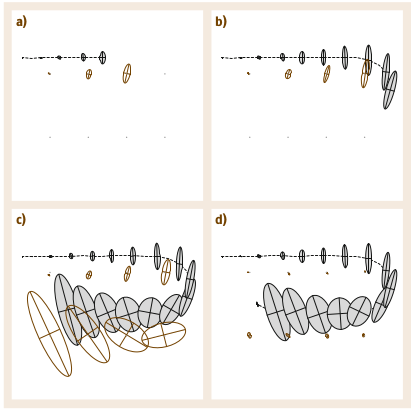
\includegraphics[width=.9\linewidth]{pictures/03/ekf}
  \caption{EKF SLAM example}
  \label{fig:ekfslam}
\end{figure} 

However, it has its drawbacks. Due to the nature of the covariance matrix, every update step takes a quadratic time, thus making the feature number low (less than 1000 features) \citeslam{Thrun2005}.

Because the number of features needs to remain low, \emph{data association} tends to become more difficult. Data association is matching the most likely measurement to a specific landmark. EKF is generally more fragile to other methods to incorrect data associations. Therefore EKF SLAM algorithms are not particularly scalable to larger problems.

Modern EKF algorithms implement some features to avoid the issues of the earliest approaches. Furthermore, there is another approach called \textbf{Extended Information Filter (EIF)} described by the information matrix and the information vector \citeslam{Bailey2006b, Stachniss2014c}:
\begin{gather}
  \Omega = \Sigma^{-1} \\
  \zeta = \Sigma^{-1}\mu
  \label{eq:eif}
\end{gather}

This approach is interesting because many of the off--diagonal components of the \emph{normalized} information matrix are $0$, making it a sparse matrix and making update steps more efficient.

\subsection{Particle Filter SLAM} \label{sub:particle}

The particle filter approach seeks to sample the probability distribution with discrete states (known as particles), instead of approximating using Gaussians. Each particle represents the posterior belief of the system and has associated a weight,$w$, that corresponds to the likelihood of that particle \citeslam{Stachniss2014d, Thrun2005}:
\begin{equation}
  \chi_t = \{<x^{[j]},\;w^{[j]}>\}\quad j=1,\ldots,J
  \label{eq:pf}
\end{equation}  

The steps of the particle filter are:
\begin{enumerate}
  \item \textbf{Sample from proposal distribution}: it is represented by letter $\pi$ and in this case it is coincident with the motion model distribution:
  \begin{equation}
    x_t^{[j]} \sim \pi(x_t|\ldots) = p(x_t|x_{1:t-1}, u_t) 
    \label{eq:pfmotion}
  \end{equation}  

  After this step, the predicted particles are obtained, $\overline{\chi}_t$, which is the representation of $\overline{bel}(x_t)$ in the Bayes Filter.

  \item \textbf{Calculate the weights for each particle}: With the particles in $x_t$, the weight of each one is calculated by dividing the target distribution with the proposal wich is proportional to the observation model:
  \begin{equation}
    w_t^{[j]} = \frac{target}{proposal} \propto p(z_t|x_t^{[j]}) 
    \label{eq:pfobs}
  \end{equation}  

  \item \textbf{Resampling}: In this step a sample $i$ is drawn with probability $w_t^{[i]}$ and this process is repeated $J$ times. In this last step, the more likely particles are kept whereas the ones that are more unlikely get discarded.
\end{enumerate}  

The problem of particle filters applied to SLAM is that the state space tends to have a notable size (\autoref{eq:combinedstate}). Particle filters scale exponentially, therefore if the number of landmarks is considerable the problem becomes untractable. 

\textbf{FastSLAM}, originally developed by \citeslam{Montemerlo2002} is an algorithm that exploits the independence among the different map features \autoref{fig:mapindep}. In the original implementation, it only applied to feature based maps.
\begin{figure}[t]
  \centering
  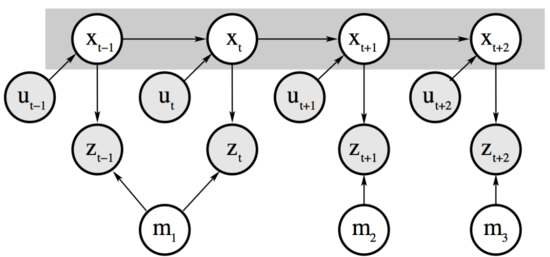
\includegraphics[width=\linewidth]{pictures/03/mapindep}
  \caption[Landmarks are independent from each other]{Conceptual view of how each landmark is disconnected from the rest}
  \label{fig:mapindep}
\end{figure}  

The belief at time $t$ can be factored as:
\begin{equation}
  p(x_{0:t},m|z_{1:t},u_{1:t}) = p(x_{0:t}|z_{1:t},u_{1:t})\cdot \prod\limits_{i=1}^{N}p(m_i|x_{0:t}, z_{1:t})
  \label{eq:rao}
\end{equation}  
where each of the landmarks represents a 2--dimension gaussian distribution with mean and covariance $\mu_{t,n}^{[j]}$ and $\Sigma_{t,n}^{[j]}$ respectively. Due to a technique called \emph{Rao--Blackwellization} for every particle the map posteriors can be estimated independently.

The posterior estimation is done as follows:
\begin{enumerate}
  \item \textbf{Sampling}: A set of particles if sampled from the motion model:
  \begin{equation}
    x_t^{[j]} \sim p(x_t|x_{t-1}^{[j]},u_t)
    \label{eq:slamsamplemotion}
  \end{equation}  

  \item \textbf{Update the observed features estimates}: This is done for each particle and the update is done employing the EKF. For any unobserved feature the gaussian remains the same:
  \begin{equation}
    \langle \mu_{t,n}^{[j]},\; \Sigma_{t,n}^{[j]}\rangle = \langle \mu_{t-1,n}^{[j]},\; \Sigma_{t-1,n}^{[j]}\rangle
    \label{eq:simpleupdate}
  \end{equation}  

  \item \textbf{Resampling}: First the weights are calculated with $p(x_{0:t}|z_{1:t},u_{1:t})$ as target and $p(x_{0:t}|z_{1:t-1},u_{1:t})$ as proposal distributions. Each weight $w_t^{[j]}$ can be obtained via \citeslam{Thrun2005, Tobergte2013}:
  \begin{equation}
    \begin{split}
    w_t^{[j]} & = \frac{target(x^{[j]})}{proposal(x^{[j]})} = \frac{p(x^{[j]}_{0:t}|z_{1:t},u_{1:t})}{p(x^{[j]}_{0:t}|z_{1:t-1},u_{1:t})}\\
              & = \frac{\eta p(z_t|x^{[j]}_{0:t},z_{1:t-1})\cdot p(x^{[j]}_{0:t}|z_{1:t-1},u_{1:t})}{p(x^{[j]}_{0:t}|z_{1:t-1},u_{1:t})} \\
              & = \eta p(z_t|x^{[j]}_{0:t},z_{1:t-1}) \\
              & = \eta\!\int\!  p(z_t|x^{[j]}_{0:t},z_{1:t-1},m_i)\cdot p(m_i|x^{[j]}_{0:t},z_{1:t-1})\cdot \mathrm{d}m_i \\
              & = \eta\!\int\!  p(z_t|x^{[j]}_{0:t},m_i)\cdot p(m_i|x^{[j]}_{0:t},z_{1:t-1})\cdot \mathrm{d}m_i
    \end{split}
  \end{equation}
\end{enumerate}  

Both probability distributions inside the integral can be approximated by Gaussian distributions and the weights can be computed with an EKF. After obtaining the weights for each particle, the new set is created being the particles with bigger weights more likely to 'survive' to the next round.

The FastSLAM algorithm has some notable properties \citeslam{Montemerlo2002, Tobergte2013}: \begin{enumerate*} \item it solves both full and online SLAM problems, \item each particle can make its own data association hypothesis and \item it is possible to implement it very efficiently \end{enumerate*}.

Apart from the feature--based FastSLAM, there exists a Grid--Map based implementation of the algorithm, which is the basis for the \textbf{GMapping} algorithm that will be explained in \autoref{sub:gmapping}.

\subsection{Graph--based SLAM}\label{sub:graphslam}

The last of the approaches that will be discused in this thesis is the \textbf{Graph--based SLAM}. The intuition behind this algorithm is as follows \citeslam{Stachniss2014e}:
\begin{itemize}
  \item \textbf{Graph}: Corresponds to the whole SLAM problem.

  \item \textbf{Nodes}: Correspond to landmarks and robot locations.

  \item \textbf{Edges}: Correspond to spatial constraints due to motion or observations.
\end{itemize}  

The whole purpose of the Graph SLAM is therefore to find a node distribution that minimizes the measurement errors.

Generally, Graph--based SLAM algorithms have the structure shown in \autoref{fig:graphslam}, where the front--end takes the measurements are obtained by \emph{matching} observations, and the backend, where given the measurements it builds the constraints and optimizes the graph.
\begin{figure}[htb]
  \centering
  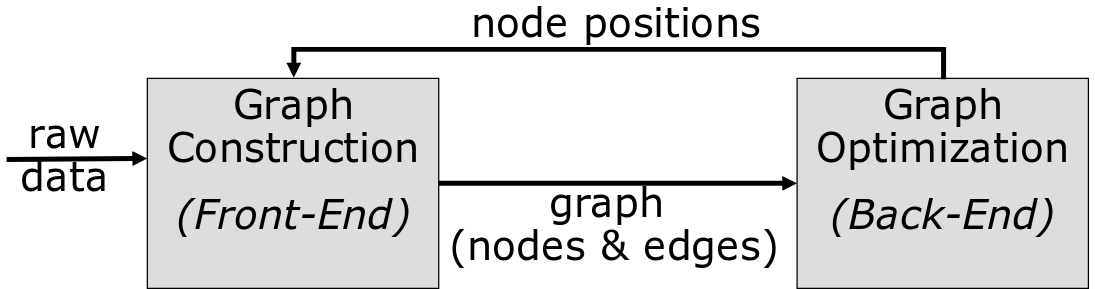
\includegraphics[width=\linewidth]{pictures/03/graphslam}
  \caption{Graph--based SLAM structure}
  \label{fig:graphslam}
\end{figure}  

\parunder{Backend:} The definition of the optimization is described in the following paragraphs \citeslam{Grisetti2010}. The vector describing the pose of every node $i$ is defined $x = (x_1,x_2,\ldots,x_N)^T$. $z_{ij}$ and $\Omega_{ij}$ are the mean of the measurement and the information matrix from node $i$ to $j$. $\hat{z}_{ij}(x_i,x_j)$ is the prediction of a measurement given nodes $i$ and $j$.

Therefore an error function can be defined as:
\begin{equation}
  e_{ij} = z_{ij} - \hat{z}_{ij}(x_i,x_j)
  \label{eq:error}
\end{equation}  

$\mathbf{F}(x)$ is the negative log likelihood:
\begin{equation}
  \mathbf{F}(x) = \sum\limits_{\langle i,j \rangle}e_{ij}^T\cdot \Omega_{ij}\cdot e_{ij}
  \label{eq:fx}
\end{equation}  
and the objective is to minimize $\mathbf{F}(x)$:
\begin{equation}
  x^* = argmin\;\mathbf{F}(x)
  \label{eq:minfx}
\end{equation}  

\autoref{eq:minfx} corresponds to a \textbf{non--linear least squares} problem and it can be solved using well-known methods such as gradient descent, Newton--Gauss, Lavenberg--Marquardt \citeslam{Grisetti2010}.

Generally, this is done by linearizing the error function with a first order Taylor expansion around the initial guess $\breve{x}$:
\begin{equation}
  \begin{split}
    e_{ij}(\breve{x}_i + \Delta x_i, \breve{x}_j + \Delta x_j) & = e_{ij}(\breve{x} + \Delta x) \\
                                                                & \approx e_{ij} + J_{ij}\Delta x
  \end{split}  
  \label{eq:taylorerror}
\end{equation}
where $J_{ij}$ is the jacobian matrix.

In terms of $F_{ij}$ the equation results in:
\begin{equation}
  \begin{split}
    F_{ij}& (\breve{x}+\Delta x)\\
          & = (e_{ij}(\breve{x} + \Delta x)^T\cdot \Omega_{ij}\cdot e_{ij}(\breve{x} + \Delta x) \\
          & \approx (e_{ij} + J_{ij}\Delta x)^T\cdot \Omega_{ij}\cdot (e_{ij} + J_{ij}\Delta x) \\
          & = e_{ij}^T\Omega_{ij}e_{ij} + 2e_{ij}^TJ_{ij}\Delta x + \Delta x J_{ij}^T \Omega_{ij} J_{ij} \Delta x^T \\
          & = c_{ij} + 2b_{ij}\Delta x + \Delta x^T H_{ij} \Delta x
  \end{split}  
  \label{eq:fij}
\end{equation}

The function $\mathrm{F}(x)$ then becomes:
\begin{equation}
  \begin{split}
    \mathbf{F}(\breve{x}+\Delta x) & = \sum\limits_{\langle i, j \rangle} F_{ij}(x + \Delta x)\\
                                   & \approx \sum\limits_{\langle i, j \rangle} c_{ij} + 2b_{ij}\Delta x + \Delta x^T H_{ij} \Delta x\\
                                   & = \mathbf{c} + 2\mathbf{b}^T\Delta x + \Delta x^T \mathbf{H} \Delta x
  \end{split}  
  \label{eq:fxtaylor}
\end{equation}

\autoref{eq:fxtaylor} can be minimized by solving the linear system:
\begin{equation}
  \mathbf{H}\Delta x^* = -\mathbf{b}
  \label{eq:linearsolve}
\end{equation} 
and therefore the solution becomes:
\begin{equation}
  x^* = \breve{x} + \Delta x^*
  \label{eq:solution}
\end{equation} 

\parunder{Frontend:} The frontend of the Graph--based SLAM obtains the measurements by performing a \textbf{scan--matching} of current sensor data with previous points. The algorithms that tackle this problem are \textbf{Iterative Closest Point (ICP)}, \textbf{Correlative matching}, \textbf{Normal Distributions Transform (NDT)} among many others.

Graph SLAM algorithms have 2 key advantages \citeslam{Tobergte2013} in comparison with EKF SLAM: The update of the map is constant in time and the memory utilization grows linearly. However, the optimization step is resource consuming.

One of the features of these algorithms is that they serve for both 2D and 3D maps \citeslam{Grisetti2010}. The 'only' change that has to be made is to substitute the laser scans with 3D pointclouds. In fact \autoref{fig:slam} was built using a Graph--based SLAM algorithm.

In the past years, Graph SLAM algorithms have been subject to profound research and have become the state--of--the--art algorithms in this field \citeslam{Thrun2005, Tobergte2013}. Some of the biggest SLAM maps have been created using this approach and contain up to 10\textsuperscript{8} features.

\section{Open-source SLAM algorithms}

Fortunately, these algorthms have already been implemented in software packages and many of them are available in the open--source community. What is more, due to the success of the ROS ecosystem, generally SLAM algorithms come bundled with ROS libraries, thus making them easier to interface.

In the following pages, the main algorithms used to develop the SLAM systems of both the Nexus Robot and the PEV will be described.

\subsection{SLAM Gmapping} \label{sub:gmapping}

As it was mentioned on \autoref{sub:particle}, \textbf{Gmapping} is a particle filter SLAM variant that employs grid maps instead of feature--based maps \citeslam{Grisetti2005, Grisetti2007}, that incorporates some improvements to the original algorithms:
\begin{itemize}
  \item \textbf{Scan--matching}: Before applying the particle filter, the pose is corrected using a scan--matcher to maximize the likelihood of the current pose and map:
  \begin{equation}
    x_t^* = \mathop{argmax}_{x_t}\{p(z_t|x_t,m_{t-1})p(x_t|u_t,x^*_{t-1})\}
    \label{eq:scanmatch}
  \end{equation}  

  \item \textbf{Improving the proposal distribution}: Recalling from \autoref{sub:particle}, the importance weights are a result of the ratio between the target distribution $p(x_{0:t}|z_{1:t},u_{1:t})$ and the proposal $\pi(x_{0:t}|z_{1:t},u_{1:t})$. Gmapping computes this proposal taking into account the most recent scan, thus improving accuracy:
  \begin{equation}
    p(x_t|m_{t-1}^{[j]},x^{[j]}_{t-1},z_t,u_{t})=\frac{p(z_t|m_{t-1}^{[j]},x_t)p(x_t|x_{t-1}^{[j]},u_t)}{p(z_t|m_{t-1}^{[j]},x_{t-1}^{[j]},u_t)}
    \label{eq:improvedprop}
  \end{equation}

  \item \textbf{Adaptive resampling}: Even though resampling is necessary since the number of particles is finite and the less likely ones must be removed, the process might also remove good particles. Therefore Gmapping computes the following parameter:
  \begin{equation}
    N_{eff} = \frac{1}{\sum_{i=1}^{N}(\tilde{w}^{[j]})^2}
    \label{eq:neff}
  \end{equation}
  where $\tilde{w}^{(i)}$ is the normalized weight. The algorithm will do a resampling step whenever $N_{eff}$ drops below $N/2$, being $N$ the number of particles. Thus, the resampling operation is done when needed.
\end{itemize}  

Gmapping is one of the first open--source alogorithms to appear on the ROS ecosystem\footnote{http://wiki.ros.org/gmapping} and it blends naturally with the Navigation Stack. Some of the main characteristics of this ROS package are:
\begin{itemize}
  \item \textbf{Subscribed topics}: The main topics are \texttt{/tf} to obtain the rigid body transforms and \texttt{scan} to obtain the laser messages. The necessary transforms are:
  \begin{itemize}
    \item \texttt{laser\_frame}\arrow\texttt{base\_link}. Transformation between the frame of the range sensor and the main frame of the robot.
    \item \texttt{base\_link}\arrow\texttt{odom}. Transformation between the base frame and an odometry frame.
  \end{itemize}  

  \item \textbf{Published topics}: Gmapping publishes the \textbf{occupancy grid map} to the \texttt{/map} topic.

  \item \textbf{Provided transforms}: Gmapping provides the transform \texttt{map}\arrow\texttt{odom} with the robot's pose within the map.

  \item \textbf{Parameters}: \autoref{tab:gmapping} shows a list of the main parameters of the algorithm. The full list can be found on the \href{http://wiki.ros.org/gmapping}{ROS Wiki}
\end{itemize}

\begin{table}[htb]
  \centering
  \resizebox{\textwidth}{!}{%
    \begin{tabular}{lcl}
      \hline
      \textbf{Name} & \textbf{Default} & \textbf{Description} \\ \hline
      $\sim$base\_frame & "base\_link" & Frame attached to mobile base \\ \hline
      $\sim$map\_frame & "map" & Frame attached to the map \\ \hline
      $\sim$odom\_frame & "odom" & Frame attached to odometry \\ \hline
      $\sim$map\_update\_interval & 5 & Time (s) between map updates \\ \hline
      $\sim$maxUrange & 80 & Usable range of the laser \\ \hline
      $\sim$iterations & 5 & Max iterations of the scanmatcher \\ \hline
      $\sim$linearUpdate & 1.0 & Process scan every x meters \\ \hline
      $\sim$angularUpdate & 0.5 & Process scan every x radians \\ \hline
      $\sim$particles & 30 & Number of particles in the filter \\ \hline
      $\sim$resampleThreshold & 0.5 & $N_{eff}$ limit to resample \\ \hline
    \end{tabular}%
  }
  \caption{Gmapping main parameters}
  \label{tab:gmapping}
\end{table} 

\subsection{Hector SLAM} \label{sub:hector}

Hector SLAM is another ROS--based SLAM approach that fully integrates with the Navigation Stack and that is capable of performing 3D motion estimation \citeslam{Kohlbrecher2011}. \autoref{fig:hector} shows the Hector SLAM system overview.
\begin{figure}[htb]
  \centering
  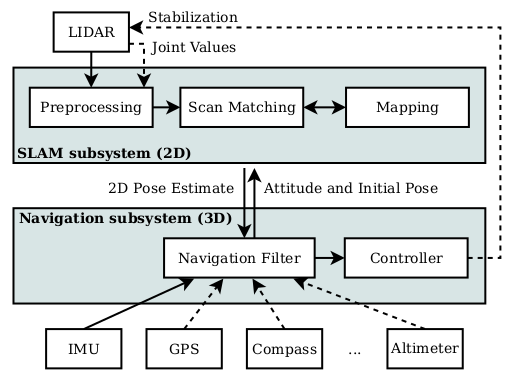
\includegraphics[width=\linewidth]{pictures/03/hector}
  \caption{Hector SLAM overview}
  \label{fig:hector}
\end{figure}  

There are 2 clear layers in the system:
\begin{itemize}
  \item \textbf{SLAM subsystem}: It reads the scans from the laser, performs the scan matching opperation and stores the results on a grid--map in 2 dimensions. This algorithm does not divide the SLAM between frontend and backend as it was explained in \autoref{sub:graphslam}: instead, it relies on the scan--matching operation to update the map. Maps are divided into multiple resolution layers to gain more consistency in the localization.

  \item \textbf{Navigation subsystem}: It estimates the 6D pose by employing an EKF: the 2D pose given by the SLAM layer is augmented with inertial sensors or GPS. The 3D state vector is defined as $\mathbf{x}=\{\mathbf{\Omega}^T\;\mathbf{p}^T\;\mathbf{v}^T\}^T$ with $\mathbf{\Omega} = \{\phi,\theta,\varphi\}^T$ the roll--pitch--yaw angles, $\mathbf{p}=\{p_x,p_y,p_z\}^T$ the position and $\mathbf{v}=\{v_x,v_y,v_z\}$ the velocity in the navigation frame.
\end{itemize}  

Because it does not perform any graph optimization on the backend, this algorithm is best suited for smaller scale scenarios with less loop closures to execute. However, this algorithm has one interesting feature which is the possibility of not using odometry. 

With regards to the \href{http://wiki.ros.org/hector_slam}{Hector SLAM ROS API}, here are some of the main features of this package:
\begin{itemize}
  \item \textbf{Subscribed topics}: The main topics are \texttt{/tf} and \texttt{scan} like in Gmapping. The necessary transforms are:
  \begin{itemize}
    \item \texttt{laser\_frame}\arrow\texttt{base\_link}. Transformation between the frame of the range sensor and the main frame of the robot.
    \item \texttt{base\_link}\arrow\texttt{odom}. Only if the odom frame is provided by an external node.
  \end{itemize}  

  \item \textbf{Published topics}: Hector SLAM publishes the map to \texttt{/map} and the pose of the robot to \texttt{/poseupdate}.

  \item \textbf{Provided transforms}: Hector SLAM provides the transform \texttt{map}\arrow\texttt{odom} with the robot's pose within the map.

  \item \textbf{Parameters}: \autoref{tab:hector} shows a list of the principal parameters available for Hector SLAM
\end{itemize}
\begin{table}[htb]
  \centering
  \resizebox{\textwidth}{!}{%
    \begin{tabular}{lcp{6cm}}
      \hline
      \textbf{Name} & \textbf{Default} & \textbf{Description} \\ \hline
      $\sim$base\_frame & "base\_link" & Frame attached to mobile base \\ \hline
      $\sim$map\_frame & "map" & Frame attached to the map \\ \hline
      $\sim$odom\_frame & "odom" & Frame attached to odometry. It can be set to "base\_link" when no odometry is provided \\ \hline
      $\sim$map\_update\_distance\_thresh & 0.4 & Threshold for map update after linear motion \\ \hline
      $\sim$map\_update\_distance\_thresh & 0.9 & Threshold for map update after angular motion \\ \hline
      $\sim$map\_multi\_res\_levels & 3 & Number of grid levels for the map \\ \hline
      $\sim$laser\_min\_dist & 0.4& Min distance to consider a scan measurement \\ \hline
      $\sim$laser\_max\_dist & 30 & Max distance for a scan measurement \\ \hline
      $\sim$pub\_map\_odom\_transform & True & Determine if \texttt{map}\arrow\texttt{odom} transform should be published by the system \\ \hline
      $\sim$scan\_subscriber\_queue\_size & 5 & Queue for the scan measurements \\ \hline
    \end{tabular}%
  }
  \caption{Hector SLAM main parameters}
  \label{tab:hector}
\end{table} 

\subsection{Google Cartographer} \label{sub:cartographer}

\href{https://google-cartographer.readthedocs.io/en/latest/}{Cartographer} is a relatively recent SLAM package (2016) developed by Google \citeslam{Hess2016a}, that aims at providing real--time 2D mapping in indoor environments.

Cartographer is an example of a Graph--based SLAM algorithm with 2 definite layers (\autoref{fig:cartographersch}):
\begin{itemize}
  \item \textbf{Local SLAM}: The local SLAM matches every scan with a small portion of the world called submap. To perform that matching it employs the Ceres solver \citeslam{ceres-solver}.

  \item \textbf{Global SLAM}: Matching scans against a submap accumulates errors over time. That is why every few seconds Cartographer takes those submaps with their underlying constraints and performs a loop--closure optimization employing once again the Ceres--solver.
\end{itemize}

\begin{figure}[t]
  \centering
  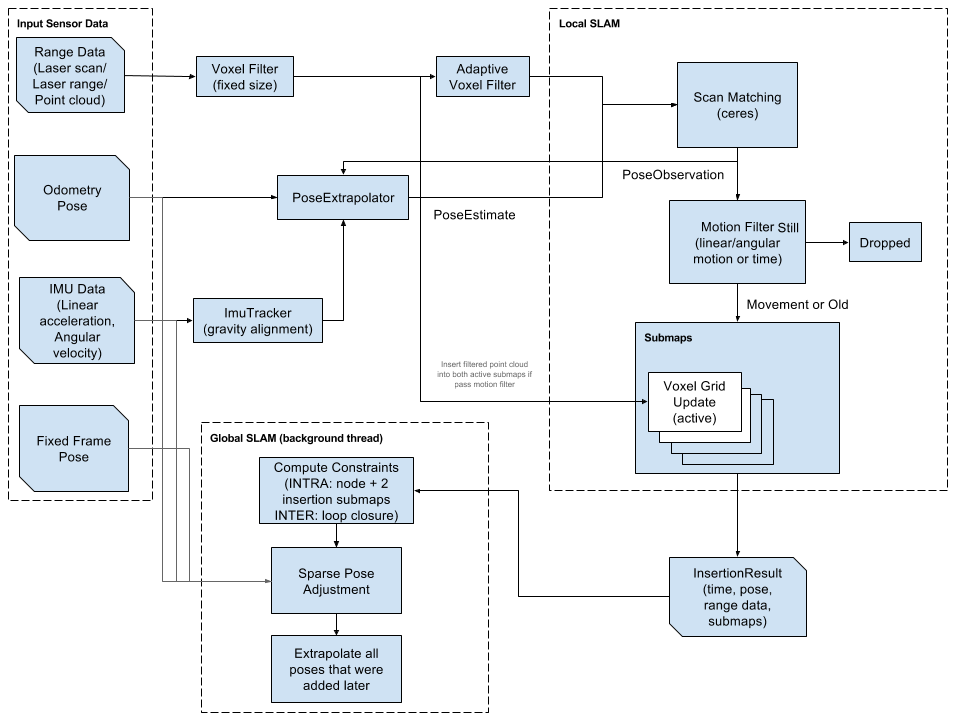
\includegraphics[width=.9\linewidth]{pictures/03/cartographersch}
  \caption{Cartographer system overview}
  \label{fig:cartographersch}
\end{figure}

As of July 2018, Cartographer provides both 2D and 3D SLAM and localization options with a extense variety of sensors that can be added: 2D/3D LIDARs, IMU, odometry information and GPS among others.

Cartographer provides as well \href{https://google-cartographer-ros.readthedocs.io/en/latest/}{ROS wrappers} that allow its use with the existing stack of packages:
\begin{itemize}
  \item \textbf{Subscribed topics}: The topics that it subsribes are (\autoref{tab:cartographertopics}):   
    \begin{table}[htb]
      \centering
      \resizebox{\textwidth}{!}{%
        \begin{tabular}{llp{6cm}}
          \hline
          \textbf{Topic} & \textbf{Message} & \textbf{Description} \\ \hline
          scan & sensor\_msgs/LaserScan & Planar laser scanners \\ \hline
          echoes & sensor\_msgs/MultiEchoLaserScan & Axially rotating planar laser scanners \\ \hline
          points2 & sensor\_msgs/PointCloud2 & 2D/3D pointclouds \\ \hline
          imu & sensor\_msgs/Imu & Optional in 2D, required in 3D \\ \hline
          odom & nav\_msgs/Odometry & Optional in both modes \\ \hline
        \end{tabular}%
      }
      \caption{Cartographer subscribed topics}
      \label{tab:cartographertopics}
    \end{table}
  
  \item \textbf{Published topics}: \texttt{scan\_matched\_points2} with the pointcloud and \texttt{submap\_list} with a list of all submaps.

  \item \textbf{Transforms}:
    \begin{itemize}
      \item \textbf{Required}: \texttt{tracking\_frame}\arrow\texttt{published\_frame}
      \item \textbf{Provided}: \texttt{published\_frame}\arrow\texttt{map\_frame}
    \end{itemize}    

  \item \textbf{Parameters}: The amount of features and parameters that can be tweaked is considerable as it is shown below:
  \begin{itemize}
    \item \textbf{General options}: Main sensors, the frame names and SLAM main options.
    \item \textbf{Map builder}: SLAM method (2D or 3D) and the number of threads.
    \item \textbf{Trajectory builder}: Options for the scan--matcher and the trajectory.
    \item \textbf{Pose graph}: Options for the global optimizer
  \end{itemize}  
\end{itemize}

After the information given above, it can be noted that Cartographer is a powerful tool that enables SLAM in relatively large areas. A notable example is the mapping of the whole first floor of the Deutsches Museum as shown in \autoref{fig:cartographerdeutsches}.
\begin{figure}[htb]
  \centering
  \frame{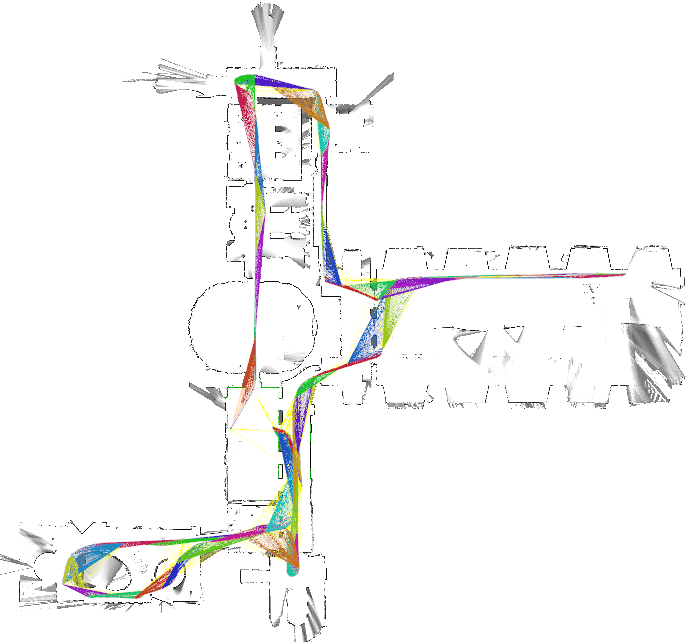
\includegraphics[width=.9\linewidth]{pictures/03/deutsches2}}
  \caption[2D map with Cartographer]{2D map of the Deutsches Museum done with Cartographer}
  \label{fig:cartographerdeutsches}
\end{figure}  

\subsection{Autoware and Normal Distributions Transform (NDT)} \label{sub:autoware}

The last software tool employed is \href{https://github.com/CPFL/Autoware}{Autoware}, a ROS--based open--source software package aiming at developing outdoor autonomous car technologies \citeslam{Kato2015, Kato2018}. 

\begin{figure}[htb]
  \centering
  \frame{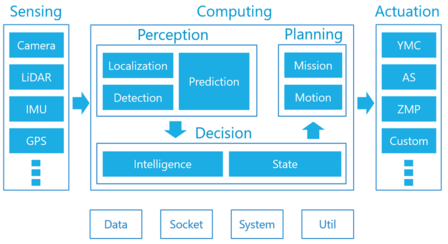
\includegraphics[width=.9\linewidth]{pictures/03/autowaresch}}
  \caption{Autoware functionalities}
  \label{fig:autowaresch}
\end{figure}

It is not a SLAM algorithm per--se, but a standalone module that provides libraries for motion planning, perception and actuation (\autoref{fig:autowaresch}). Among the perception packages several 3D SLAM and localization algorithms can be found, that merge 3D LiDAR, IMU and GPS sensors among others.

The 3D SLAM algorithms rely on scan--matching (like in Hector SLAM), and concretely they apply the 3D version of the Normal Distributions Transform (NDT) \citeslam{Biber}. After each localization, the algorithm registers the pointcloud and updates the 3D map. \autoref{fig:slam} is an example of a map built using this technique.

NDT mapping can be used with the Graphical User Interface (GUI) shown in \autoref{fig:autowaregui} or as a standalone module.
\begin{figure}[htb]
  \centering
  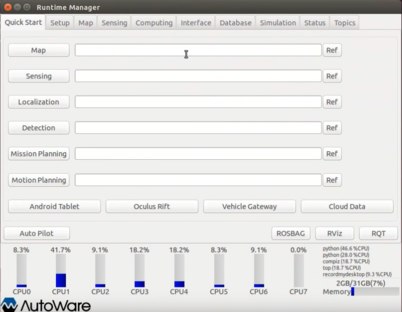
\includegraphics[width=.9\linewidth]{pictures/03/autowaregui}
  \caption{Autoware GUI}
  \label{fig:autowaregui}
\end{figure}

If used as a standalone module, the required aspects are:
\begin{itemize}
  \item \textbf{Subscribed topics}: Subscribed topics are shown in \autoref{tab:ndttopics}
    \begin{table}[htb]
      \centering
      \resizebox{\textwidth}{!}{%
        \begin{tabular}{llp{6cm}}
          \hline
          \textbf{Topic} & \textbf{Message} & \textbf{Description} \\ \hline
          points\_raw & sensor\_msgs/PointCloud2 & 3D pointcloud \\ \hline
          vehicle/odom & nav\_msgs/Odometry & Optional \\ \hline
          imu\_raw & sensor\_msgs/Imu & Optional\\ \hline
          ndt\_mapping & ConfigNdtMapping & Configuration for autoware \\ \hline
          ndt\_mapping\_output & ConfigNdtMappingOutput & Configuration for the pointcloud \\ \hline
          
        \end{tabular}%
      }
      \caption{Autoware's NDT subscribed topics}
      \label{tab:ndttopics}
    \end{table}

  \item \textbf{Published topics}: NDT mapping publishes a single topic with the 3D map of the environment called \texttt{/ndt\_map}.

  \item \textbf{Transforms}: The required transforms are \texttt{sensor\_frame}\arrow\texttt{base\_link}. 

  \item \textbf{Parameters}: Parameters are specified in \autoref{tab:ndt}

  \begin{table}[htb]
    \centering
    \resizebox{\textwidth}{!}{%
      \begin{tabular}{lcp{6cm}}
        \hline
        \textbf{Name} & \textbf{Default} & \textbf{Description} \\ \hline
        $\sim$tf\_xxx & no default & These are 6 parameters for the x, y, x, roll, pitch and yaw transform between base and map \\ \hline
        $\sim$method\_type & 0 & Specifies type of pointcloud \\ \hline
        $\sim$odom\_frame & "odom" & Frame attached to odometry. It can be set to "base\_link" when no odometry is provided \\ \hline
        $\sim$use\_imu & False & Specifies if IMU is used\\ \hline
        $\sim$imu\_upside\_down & False & Specifies if IMU is turned 180\textdegree \\ \hline
        $\sim$imu\_topic & /imu\_raw & Topic to listen IMU messages \\ \hline
        $\sim$use\_odom & False & Specifies if odometry is used \\ \hline
      \end{tabular}%
    }
    \caption{Autoware's NDT mapping main parameters}
    \label{tab:ndt}
  \end{table} 
\end{itemize}

